
\chapter{Implementation and Preliminary Results}

\section{Code Structure}

\subsection{Frontend}
The frontend implementation of Medibot utilizes ReactJS enhanced with TypeScript, which provides strong typing to improve code reliability and debuggability. The frontend architecture is meticulously designed to be modular, promoting extensive reusability and ease of maintenance. This modularity ensures that components can be reused and updated independently, facilitating scalable application development.

\begin{figure}[H]
    \centering
    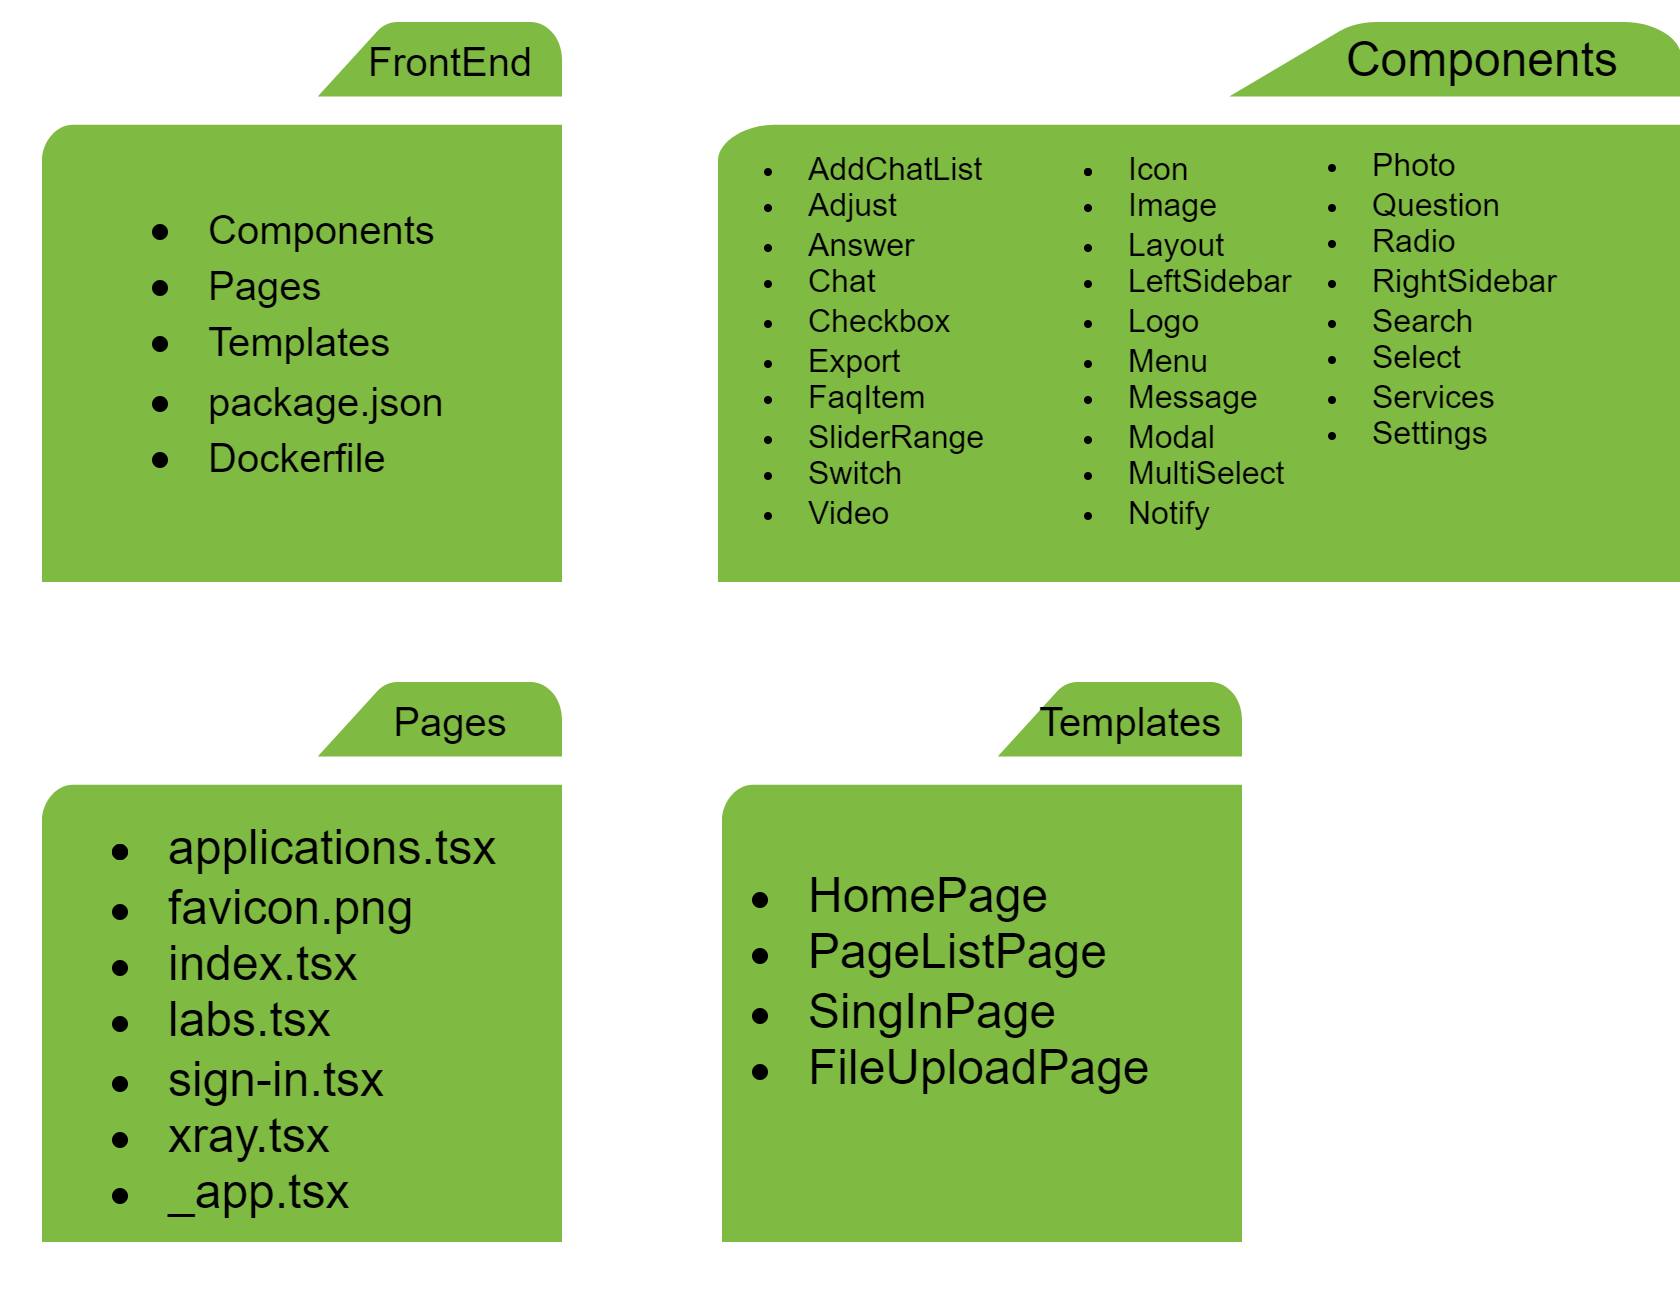
\includegraphics[width=0.8\textwidth]{./Figures/FrontendCodeStructure.png}
    \caption{Frontend Code Structure}
    \label{fig:frontend_code_structure}
\end{figure}

The frontend codebase is organized into several distinct sections:
\begin{itemize}
    \item \textbf{Components:} This directory hosts reusable UI elements such as buttons, modals, and input fields, which are standardized to maintain consistency across the application.
    \item \textbf{Pages:} Contains components that correspond to various routes within the application, like the home page, chat interface, and image upload page. These components integrate various elements from the Components and Templates directories to render comprehensive views.
    \item \textbf{Templates:} Includes layout templates used across different pages, facilitating a uniform structure and design throughout the application.
    \item \textbf{Dockerfile:} A Docker configuration file that enables the frontend to be deployed in a containerized environment, enhancing the portability and scalability of the application.
\end{itemize}

This structure not only simplifies the development process but also streamlines future enhancements and scalability by allowing developers to navigate the codebase easily, implement updates, and add new features without disrupting existing functionalities.


\subsection{Backend}
The backend of Medibot is developed using Node.js, leveraging its non-blocking I/O capabilities to handle concurrent user interactions efficiently. The backend structure is optimized for performance and scalability, making extensive use of MongoDB for data storage, which allows flexible data handling and rapid retrieval necessary for real-time applications like Medibot.

\begin{figure}[H]
    \centering
    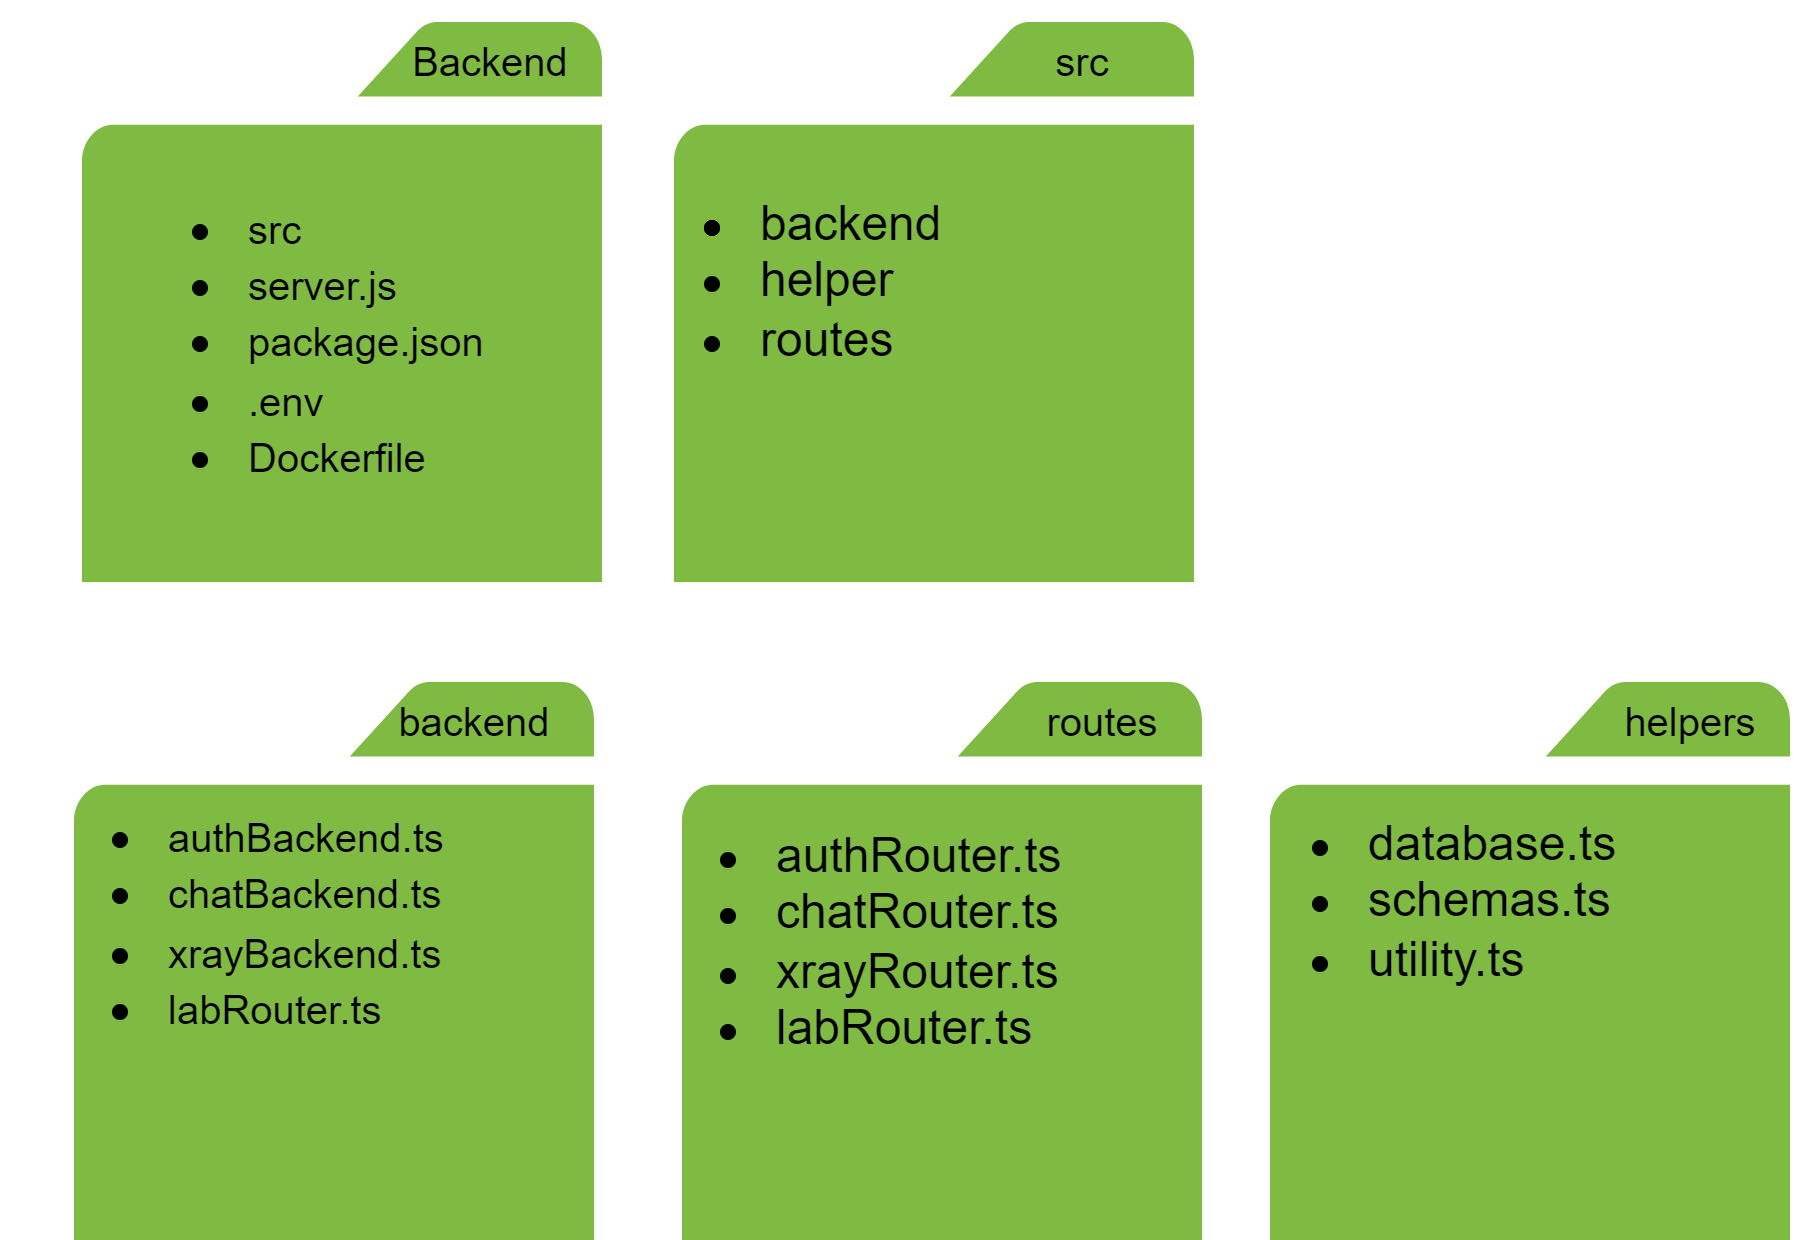
\includegraphics[width=0.8\textwidth]{./Figures/BackendCodeStructure.png}
    \caption{Backend Code Structure}
    \label{fig:backend_code_structure}
\end{figure}

The backend architecture is structured as follows:
\begin{itemize}
    \item \textbf{src:} This directory serves as the primary container for the backend code, including:
    \begin{itemize}
        \item \textbf{backend:} Houses core backend logic that handles operations such as authentication, chat management, X-ray analysis, and lab report processing.
        \item \textbf{helper:} Contains helper functions that support the backend operations by providing utility functions and database schema definitions.
        \item \textbf{routes:} Manages all the routing logic, directing requests to the appropriate controllers based on the endpoint accessed.
    \end{itemize}
    \item \textbf{server.js:} The main entry point for the backend server which initializes the application and sets up the connection to the MongoDB database.
    \item \textbf{package.json:} Specifies the project dependencies and scripts necessary for the Node.js environment.
    \item \textbf{.env:} A configuration file that stores environment-specific variables such as database credentials, ensuring sensitive data is kept secure.
    \item \textbf{Dockerfile:} Facilitates the deployment of the backend in a containerized environment, enhancing the portability and consistency of the application across different development and production setups.
\end{itemize}

This organized structure ensures that the backend remains maintainable and scalable, accommodating future expansions and functionalities seamlessly.


\subsection{Large Language Models (LLMs)}
The Large Language Models (LLMs) component is crucial to Medibot, providing the intelligent processing power needed for interacting with users and analyzing medical data. The LLMs are organized into distinct agents and tools, each serving specific functions within the Medibot system.

\begin{figure}[H]
    \centering
    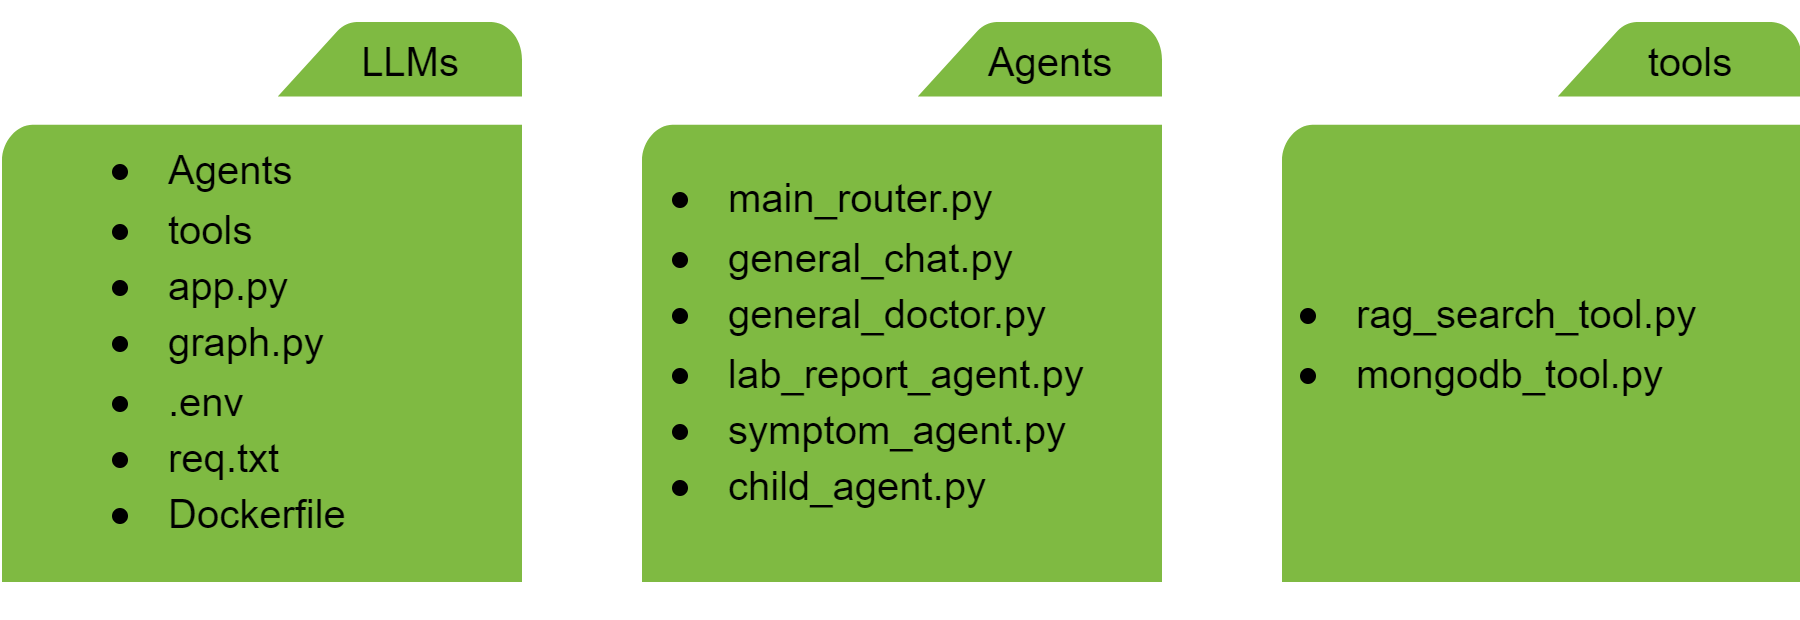
\includegraphics[width=\textwidth]{./Figures/AgentCodeStructure.png}
    \caption{Structure of LLM Agents and Tools}
    \label{fig:llm_agents_structure}
\end{figure}

\subsubsection{Agents}
The agents are specialized Python modules, each tailored to perform specific tasks:
\begin{itemize}
    \item \textbf{main\_router.py} — Directs user inquiries to the appropriate agent based on the query context.
    \item \textbf{general\_chat.py} — Handles general user interactions and queries.
    \item \textbf{general\_doctor.py} — Provides medical advice based on analyzed symptoms and user history.
    \item \textbf{lab\_report\_agent.py} — Processes and extracts information from uploaded lab reports.
    \item \textbf{symptom\_agent.py} — Specializes in identifying and categorizing symptoms described by users.
    \item \textbf{child\_agent.py} — Offers pediatric-specific advice and information, integrating guidelines from pediatric sources.
\end{itemize}

\subsubsection{Tools}
Supporting the agents are various tools that enhance their capabilities:
\begin{itemize}
    \item \textbf{rag\_search\_tool.py} — Utilizes retrieval-augmented generation to fetch and integrate external data sources for enriched responses.
    \item \textbf{mongodb\_tool.py} — Manages database interactions, facilitating data storage and retrieval from MongoDB.
\end{itemize}

\subsubsection{Infrastructure}
The LLMs operate within a Python environment, managed and isolated using Docker for consistent deployment. The structure also includes:
\begin{itemize}
    \item \textbf{app.py} — Initializes the server and sets up the application.
    \item \textbf{graph.py} — Manages knowledge graph interactions for complex data relationships.
    \item \textbf{.env} and \textbf{req.txt} — Manage environment variables and Python dependencies, respectively.
    \item \textbf{Dockerfile} — Defines the Docker container configuration to ensure environment consistency across different setups.
\end{itemize}

This layout supports Medibot’s operational needs by ensuring modular, maintainable, and scalable interactions between different components of the AI system.

\subsection{Computer Vision Models}
The Computer Vision (CV) component of Medibot is crucial for analyzing medical images such as X-rays and lab reports. This section of the system is designed for high performance and accuracy in image classification and analysis.

\begin{figure}[H]
    \centering
    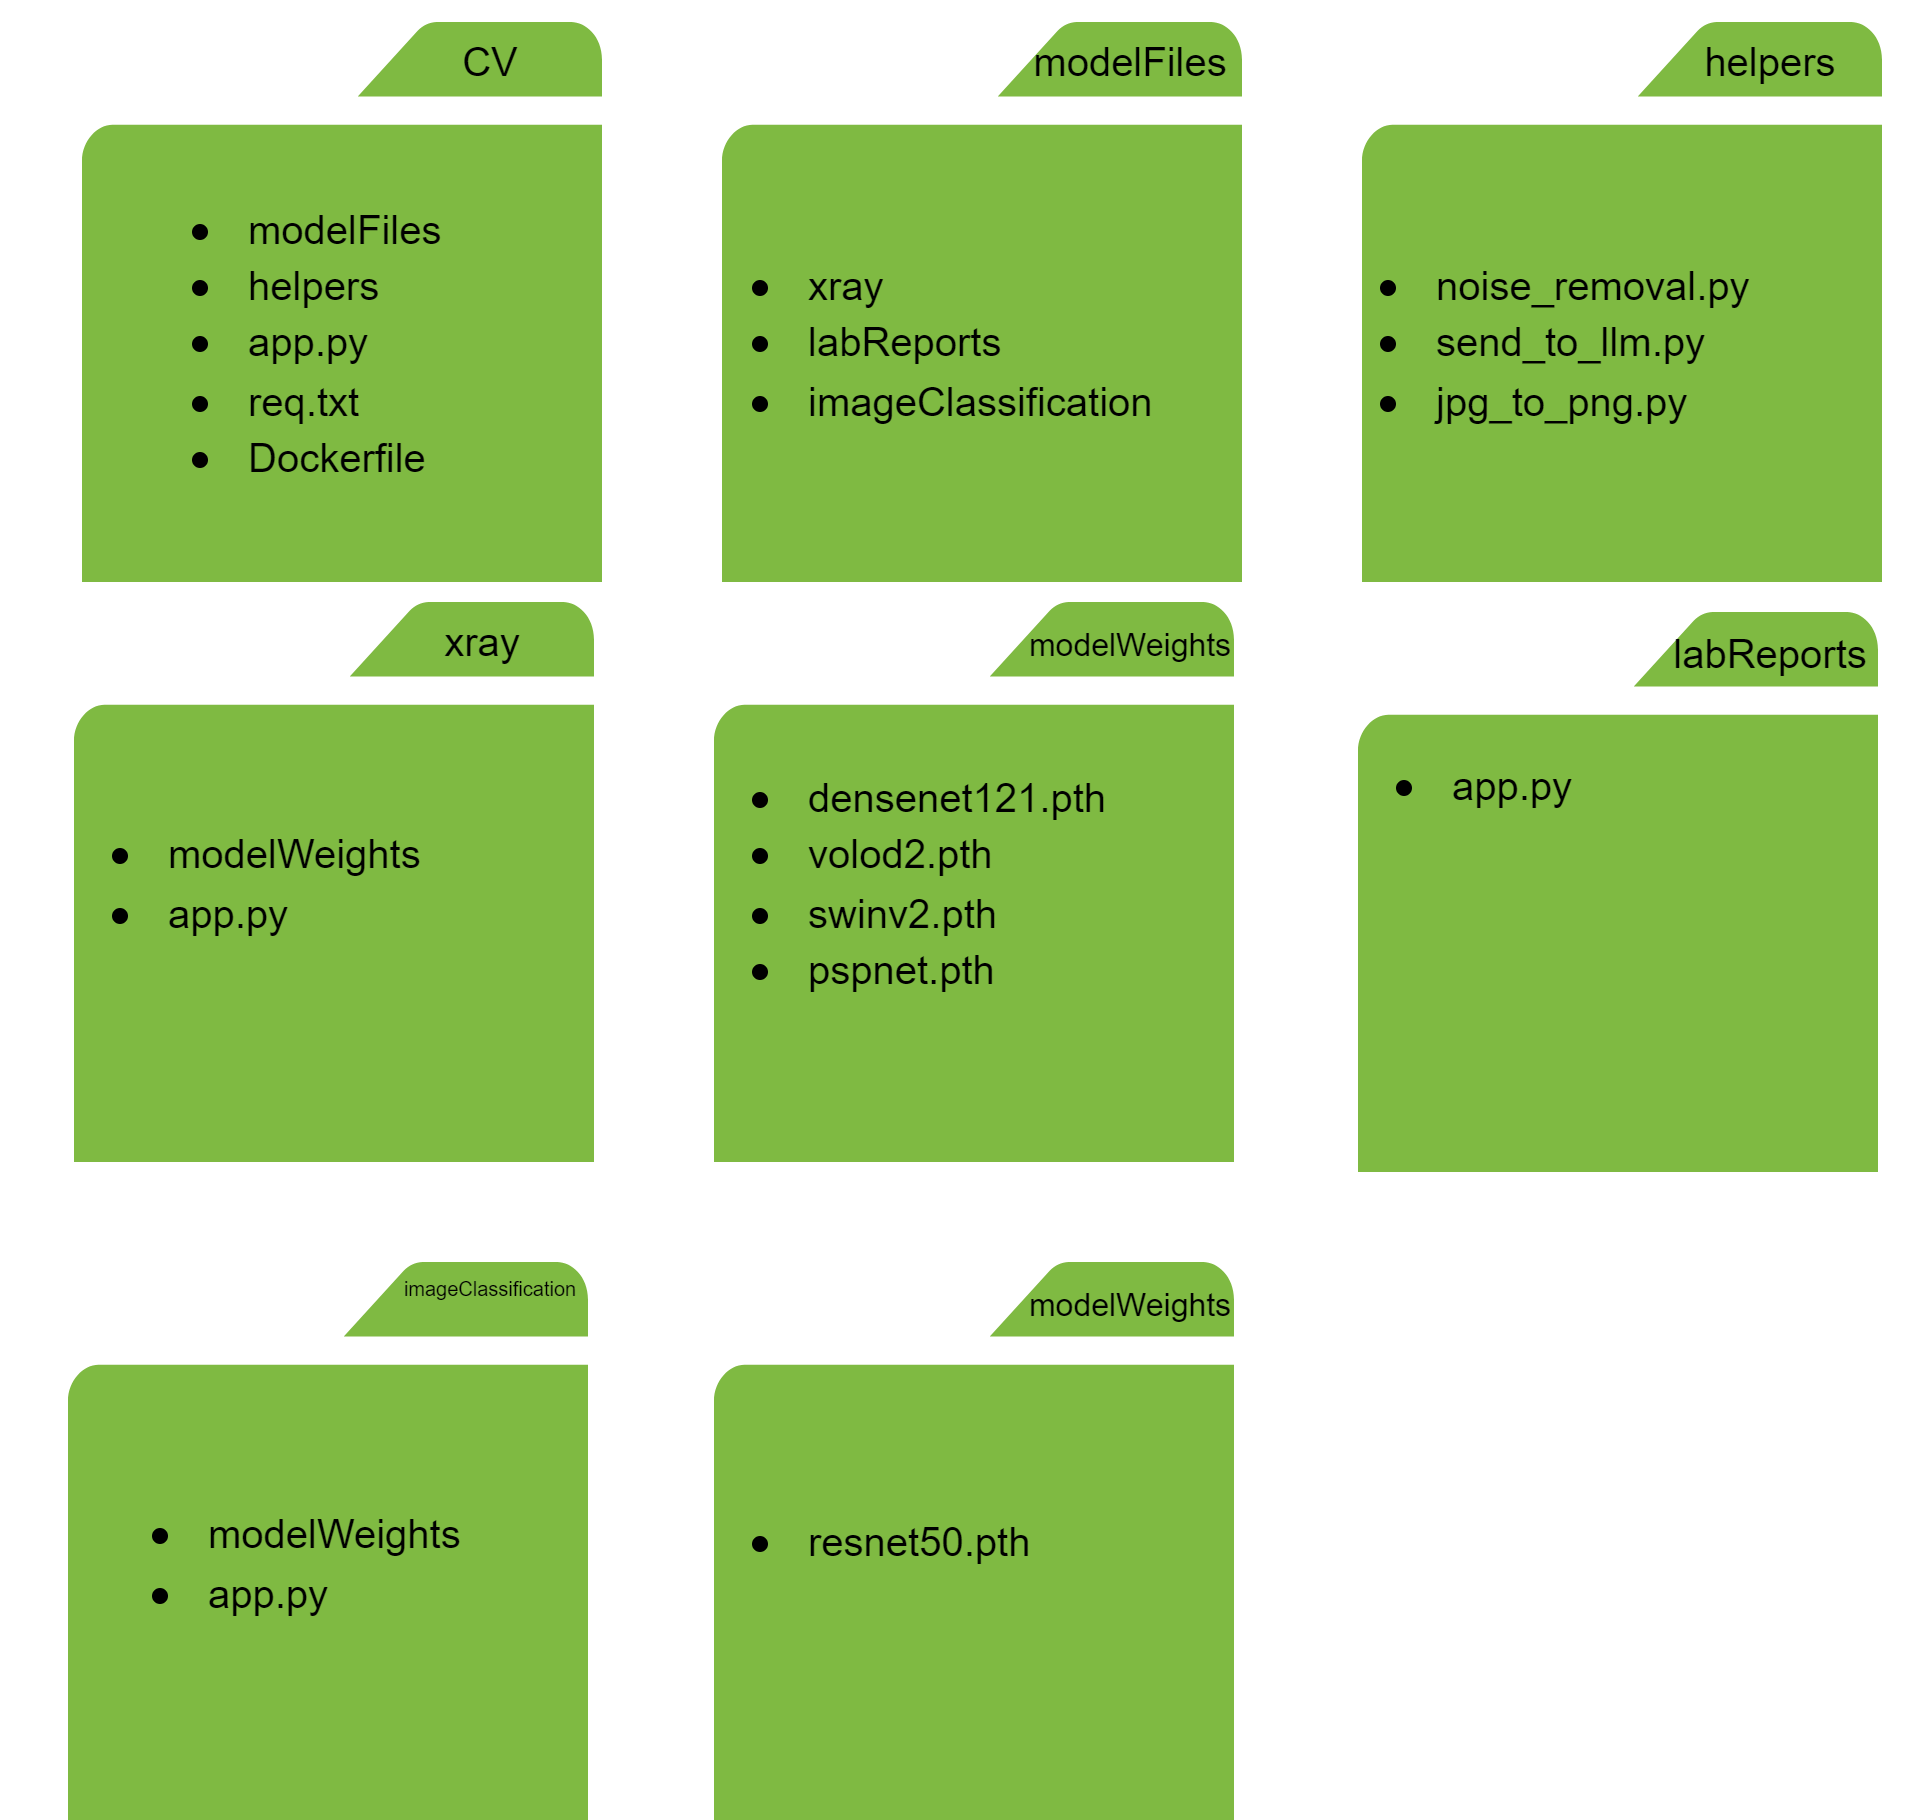
\includegraphics[width=\textwidth]{./Figures/CVCodeStructure.png}
    \caption{Computer Vision Code Structure}
    \label{fig:cv_code_structure}
\end{figure}

\subsubsection{Overview}
The CV module is structured into separate directories for managing different types of model files and their corresponding weights. It is also equipped with various helper scripts to facilitate preprocessing and integration tasks.

\subsubsection{Directories and Files}
\begin{itemize}
    \item \textbf{modelFiles:} Contains directories for different categories of model applications, including X-ray analysis, lab report processing, and general image classification.
    \item \textbf{helpers:} Includes utility scripts such as:
        \begin{itemize}
            \item \textbf{noise\_removal.py} — Enhances image quality by removing noise.
            \item \textbf{send\_to\_llm.py} — Integrates processed data with LLM components for further analysis.
            \item \textbf{jpg\_to\_png.py} — Converts images from JPG to PNG format for uniformity in processing.
            \item \textbf{boundary\_analysis.py} — This script is crucial for analyzing the boundaries within lab reports. It identifies the locations of tables and other structured data elements to ensure accurate data extraction from scanned lab reports. This is particularly important for maintaining the integrity of data during the OCR process and subsequent analyses.
        \end{itemize}
\end{itemize}

\subsubsection{Model Specifics}
\paragraph{X-ray and Image Classification Models}
These models are specially trained to identify and classify medical images with high accuracy, leveraging state-of-the-art deep learning architectures:
\begin{itemize}
    \item \textbf{DenseNet121, Volod2, Swin Transformer V2, and PSPNet} are used for detailed X-ray image analysis.
    \item \textbf{ResNet50} is utilized for broader image classification tasks, ensuring models only get their respective image for processing.
\end{itemize}

\subsubsection{Lab Reports}
The lab report directory is configured with its own application script to manage the OCR and data extraction processes, ensuring that text data from scanned lab reports is accurately converted into a structured format.

\subsubsection{Infrastructure}
The entire CV architecture is dockerized, which standardizes the development environment and ensures that the models perform consistently across different deployment platforms. Each model directory includes:
\begin{itemize}
    \item \textbf{app.py} — Main application script for running the model.
    \item \textbf{modelWeights} — Folder containing the pre-trained model weights (.pth files) used for predictions.
\end{itemize}

This organized structure not only supports scalability but also enhances the maintainability of the CV component within Medibot, ensuring efficient and accurate image processing and analysis.


\section{Data Structure and Databases}
This section details the data models and schema designs utilized in the MongoDB and Milvus databases, integral to the operation of Medibot. We discuss the integration of these databases into the backend, including indexing strategies and optimization techniques employed to enhance performance.

\subsection{MongoDB Schemas}
MongoDB, a NoSQL document-based database, is used to store user data and conversational logs. The flexibility of MongoDB's schema-less architecture allows us to adjust data structures as needed. Below are the core schemas:

\subsubsection{User Schema}
The User Schema is central to managing user information and interactions within Medibot. Fields include:
\begin{itemize}
    \item \textbf{email} - User's email address.
    \item \textbf{username} - Unique username for login.
    \item \textbf{full name} - User's full legal name.
    \item \textbf{password} - Hashed password for user authentication.
    \item \textbf{conversations} - Array of references to Conversation documents.
    \item \textbf{\_id} - MongoDB's default unique identifier.
    \item \textbf{history} - Log of past interactions and sessions.
    \item \textbf{age} - User's age, optional for demographics analysis.
    \item \textbf{gender} - User's gender, optional for personalized responses.
\end{itemize}

\subsubsection{Conversation Schema}
The Conversation Schema tracks the interactions between users and Medibot:
\begin{itemize}
    \item \textbf{user\_id} - Reference to the associated User document.
    \item \textbf{\_id} - MongoDB's default unique identifier.
    \item \textbf{messages} - Array of message objects containing text and metadata.
    \item \textbf{date} - Timestamp of the conversation start.
\end{itemize}

\subsection{Milvus Vector Database Integration}
Medibot employs the Milvus vector database to manage and facilitate fast retrieval of large-scale vector data, which is essential for features like the symptom checker. Milvus enables the efficient similarity search necessary for accurately suggesting possible medical conditions based on symptom analysis.

\subsubsection{Vector Data Structure}
The vector data in Milvus is organized into collections, where each vector represents unique symptom data and potential medical diagnoses. Below is a schematic representation of the data structure used in the symptom analysis collection in Medibot:

\begin{verbatim}
{
    "id": "<unique_vector_id>",
    "vector": ["<list_of_vector_values>"],
    "$meta": {
        "metadata": {
            "id": "<vector_id>",
            "symptoms": ["<list_of_symptoms>"],
            "diseases": "<associated_medical_condition>",
            "Source_URL": "<reference_url>"
        }
    }
}
\end{verbatim}

Each vector is stored with metadata that encapsulates the symptom details and corresponding medical conditions, enabling Medibot to predict and diagnose based on user inputs.

\subsubsection{Integration and Optimization}
Integration of Milvus within Medibot involves a Dockerized environment, ensuring easy deployment and scalability. The system employs advanced indexing techniques, such as the IVF (Inverted File) index, to optimize storage and retrieval speeds. These index settings are finely tuned to the specific requirements of the search functionality, aiming to balance accuracy and query performance effectively.

\subsubsection{Querying Vectors}
The querying of vectors utilizes Milvus's robust search functions, which support specifying search parameters like the number of nearest vectors to retrieve. This functionality underpins the symptom checker tool, where user-inputted symptom vectors are matched against the database to find the most relevant medical conditions.

\subsection{Database Integration and Performance Optimization}
Both MongoDB and Milvus are integrated into Medibot's backend via Docker containers, ensuring isolated environments and easy scalability. Indexing strategies on MongoDB include:
\begin{itemize}
    \item \textbf{Text Indexes} on user emails and usernames to speed up search operations.
    \item \textbf{Compound Indexes} on conversations to optimize retrieval by user and date.
\end{itemize}
Optimization in Milvus focuses on configuring the vector dimensions and indexing parameters to balance search accuracy and query speed.





\section{Data Processing and Generation of New Datasets}
This section details the methods and technologies employed in Medibot for processing textual and image data and for generating new datasets through advanced techniques.

\subsection{Textual Data Processing and Dataset Generation}
\subsubsection{Symptom Data Transformation}
Utilizing the NIH Medline dataset, which includes comprehensive details on various medical conditions, we extracted symptom data. This data was processed with the GPT-4 model to transform descriptive symptom information into structured bullet points, enhancing clarity and usability.

\subsubsection{Question Generation}
From the bullet-pointed symptom data, new datasets containing questions and sentences that emulate patient descriptions to a doctor were generated. We employed two models for this task:
\begin{itemize}
    \item GPT-3.5 was used to generate 10,000 questions.
    \item Llama3-70b was also used to generate an additional 10,000 questions.
\end{itemize}
These questions are designed to mimic initial patient inquiries about symptoms.

\subsubsection{Follow-up Question Generation}
To create data that could simulate follow-up questions during doctor-patient interactions, we utilized the Mixtral22b*8 model. This model processed entire records from the dataset, including symptoms, causes, and treatments, to generate 40,000 diverse follow-up questions. This enhances the dataset with a broader range of conversational AI training materials.

\subsection{Image Data Processing and Augmentation}
\subsubsection{Chest X-Ray Image Dataset}
We augmented 70\% of the Chest X-Ray-14 dataset with random filters to introduce variability, simulating more challenging real-world conditions that the AI model might encounter.

\subsubsection{Lab Report Data Integration}
For training our image classification models, we integrated:
\begin{itemize}
    \item 100 real lab reports.
    \item 3,000 documents from the company documents dataset available on Kaggle.
    \item 3,000 x-ray images from existing medical image datasets.
    \item 3,000 random images from MNIST image datasets.

\end{itemize}
This mixed dataset provides a robust training environment for the Image classifier model to recognize differentiate between X-rays, lab reports and random images.

\subsection{Combined Dataset Utilization}
The augmented textual and image datasets are each used to train specific components of Medibot's AI systems. The textual data, enriched with questions and follow-up scenarios, is crucial for training the language understanding capabilities of the LLMs. This allows Medibot to handle a wide range of user inquiries with accuracy and contextually appropriate responses.

The processed image datasets, particularly those with augmented X-ray and lab report images, are used to train and fine-tune the computer vision models within Medibot. This specialization ensures that each model excels in its respective domain, from diagnosing medical conditions based on X-ray images to accurately extracting and interpreting data from lab reports.

This approach ensures that each type of data is optimally utilized according to its relevance and contribution to the overall functionality of Medibot, enhancing the system's ability to handle diverse and realistic medical diagnostic scenarios effectively.

\section{Computer Vision Models}
\subsection{X-ray Analysis}

\subsubsection{Model Training}

The X-ray analysis within Medibot involves an advanced training regimen using multiple neural network architectures to accurately detect a range of X-ray abnormalities. Our models include DenseNet121, VoLOd2, and Swin Transformer V2, trained specifically on the NIH Chest X-ray dataset (CXR14), which consists of 112,000 images depicting various medical conditions.

\begin{itemize}
    \item \textbf{Data Preprocessing:} Before training, the X-ray images are preprocessed to mitigate common imaging issues. Adjustments are made to reduce noise from glare, correct brightness and contrast imbalances, eliminate tilt and moire patterns, and filter out Gaussian noise. These preprocessing steps are crucial for ensuring the models receive clean and standardized inputs.
    \item \textbf{Training Split:} The dataset is divided into 70\% training, 10\% validation, and 20\% testing segments. This distribution allows for comprehensive learning and rigorous assessment of the model's performance.
    \item \textbf{Model Training and Fine-tuning:} Initial training sessions are conducted over 20 epochs per model on the original NIH dataset to establish a baseline understanding. Subsequent fine-tuning is performed for an additional 5 epochs on an augmented version of this dataset, incorporating synthetic variations to simulate a wider array of X-ray scenarios. This strategy significantly raises the models' accuracy and robustness.
    \item \textbf{Additional Segmentation Model:} Alongside the classification models, a PSPNet model is trained specifically for image segmentation tasks to delineate distinct anatomical structures within the X-ray images, further enhancing the diagnostic capabilities of Medibot.
\end{itemize}

\subsubsection {Model Evaluation}

The X-ray analysis model is evaluated based on several performance metrics, including accuracy, precision, recall, and F1 score. The model's ability to detect specific abnormalities is assessed through confusion matrices and ROC curves, providing insights into its strengths and limitations.

\subsubsection {Results}

The X-ray analysis model demonstrates high accuracy in detecting common abnormalities, with precision and recall scores exceeding 90\% for pneumonia and pneumothorax. The model's performance on the test set indicates its robustness and reliability in diagnosing chest X-ray images accurately.


\subsection{Image Type Classification}

\subsubsection{Model Training}

The image type classification model within Medibot employs a ResNet50 architecture. It is designed to differentiate among three distinct types of images: X-ray images, MNIST images representing random images, and document images. The model is trained on a dataset comprising 3,000 images from each category, ensuring diverse exposure to various image types.

\begin{itemize}
    \item \textbf{Data Augmentation:} To enhance the model's ability to generalize across different conditions, data augmentation techniques are applied, introducing variations in the training dataset that reflect real-world imaging scenarios.
    \item \textbf{Model Training:} The training process extends over 30 epochs with a dataset split of 70\% training, 10\% validation, and 20\% testing. This structure ensures comprehensive learning and accurate evaluation.
    \item \textbf{Validation and Testing:} The model's performance is meticulously evaluated on the validation and test sets, focusing on accuracy, recall, precision, and F1 scores to ensure effective classification across all image types.
\end{itemize}

\subsubsection{Model Evaluation}

The model's effectiveness is quantitatively assessed through key performance metrics:

\begin{itemize}
    \item \textbf{Training Performance:} Achieved an accuracy of 97.94\%, recall of 96.24\%, and an F1 score of 96.21\%, indicating exceptional internal consistency and learning capability.
    \item \textbf{Validation Performance:} On the validation set, the model demonstrated accuracy of 97.2\%, recall of 96.9\%, and an F1 score of 96.7\%.
\end{itemize}

\subsubsection{Results}

The image type classification model proves highly effective in differentiating between X-ray, document, and random MNIST images. The high scores in precision, recall, and F1 metrics during training underscore the model's capability, while validation results confirm its practical applicability and reliability in real-world scenarios.

\section{Large Language Models (LLMs)}

\subsection{Symptom Extractor Llama3-8b}

The Symptom Extractor Llama3-8b model is fine-tuned specifically for extracting medical symptoms from user inputs. It leverages advanced natural language processing techniques to identify and parse symptoms effectively, providing crucial support for diagnostic processes.


\subsubsection{LoRA Configuration}
To enhance the model's adaptability and learning efficacy without extensive retraining, Low-Rank Adaptation (LoRA) was employed with the following parameters:
\begin{itemize}
    \item \textbf{Alpha}: 64
    \item \textbf{Dropout}: 0 (no dropout)
    \item \textbf{Target Modules}: "q\_proj", "k\_proj", "v\_proj", "o\_proj", "gate\_proj", "up\_proj", "down\_proj"
\end{itemize}

This fine-tuning approach significantly enhances the model’s capability to focus on the crucial task of symptom extraction from complex medical descriptions. The specific adjustment of target layers through LoRA enables the model to retain general linguistic capabilities while adapting to specialized tasks.

\subsubsection{Training Strategy}
The training process was meticulously designed to optimize the model's performance on symptom extraction. The detailed training prompt used is structured as follows:

\begin{verbatim}
system: You are a medical assistant specialized in extracting symptoms from sentences.
user: You will extract the symptoms from the sentence: {Input_Data}
You should only output in JSON format.
assistant: {Output_Data}
\end{verbatim}

The training infrastructure was managed using the \texttt{SFTTrainer} setup, with a strategy focused on maximizing efficiency and accuracy, demonstrated by the rigorous training parameters and results.

\subsubsection{Training Results}
The model training was completed over approximately 5 epochs, with the following detailed outcomes:

\begin{itemize}
    \item \textbf{Global Steps}: 1070
    \item \textbf{Training Loss}: 0.4649
    \item \textbf{Runtime}: 2975 seconds (approx.)
    \item \textbf{Samples per Second}: 2.879
    \item \textbf{Steps per Second}: 0.36
    \item \textbf{Total FLOPs}: \(1.549 \times 10^{17}\) (Floating Point Operations)
    \item \textbf{Epochs Completed}: 4.988
\end{itemize}

\subsection{General Medical Knowledge Llama3-70b}

The Llama3-70b model, aimed at providing detailed medical information and answering related queries, was fine-tuned using a large-scale dataset and advanced training methodologies to ensure its effectiveness in real-world applications.

\subsubsection{Training Overview}
The model was trained with an extensive set of 42,000 medical questions generated by MoE Mixtral22b*8, using an 80/10/10 split for training, validation, and testing. The training was executed over 2 epochs, achieving significant improvements in understanding and generating medically relevant content.


\subsubsection{Training Setup}
The training was orchestrated using a customized setup configured as follows:
\begin{verbatim}
Trainer:
  - Batch Size: 32 per device
  - Gradient Accumulation Steps: 4
  - Maximum Steps: 1000
  - Learning Rate: 2.5e-5
  - Warmup Steps: 5
  - Logging and Evaluation: Every 5 steps
  - Checkpoint Saving: Every 25 steps
  - Evaluation Strategy: Every 50 steps
\end{verbatim}

\subsubsection{Training Prompt}
The training prompt employed was designed to emulate professional responses typical of a medical AI assistant:
\begin{verbatim}
system: You are an AI assistant specializing in medical knowledge.
user: {Question}
assistant: {Answer}
\end{verbatim}

This setup ensures that Llama3-70b effectively learns the nuances of medical consultation, enhancing its capability to respond with accurate and contextually appropriate information.

\subsubsection{Training Results}
The training process yielded the following results:
\begin{itemize}
    \item \textbf{Global Steps}: 1000
    \item \textbf{Training Loss}: 0.6078
    \item \textbf{Runtime}: 14428.7 seconds (approx.)
    \item \textbf{Samples per Second}: 4.436
    \item \textbf{Steps per Second}: 0.069
    \item \textbf{Total FLOPs}: \(1.168 \times 10^{18}\) (Floating Point Operations)
    \item \textbf{Epochs Completed}: 1.905
\end{itemize}


\section{Quantitative Results}
Graphs for our model predicting medical conditions vs base models
\section{Qualitative Results}
Response times for each part of the website and mobile app, (Chat reply time, xray reply time, lab report reply time, login time and create account time).

